\documentclass[10pt,aspectratio=43,mathserif,dvipsnames,svgnames,x11names]{beamer}
\usepackage[UTF8]{ctex}
\usetheme{Boadilla}
\usepackage{graphics}
\usepackage{listings} 
\usepackage{mdframed}
\usepackage{clrscode}
\usepackage{wrapfig}
%算法设置
\usepackage{algorithm}  
\usepackage{algorithmicx}  
\usepackage{algpseudocode}
\floatname{algorithm}{算法}
\renewcommand{\algorithmicrequire}{\textbf{输入:}} 
\renewcommand{\algorithmicensure}{\textbf{输出:}}  
\algrenewcommand{\algorithmiccomment}[1]{ $//$ #1}
\usepackage{latexsym}
\usepackage{amsmath,amssymb,bm}
\usepackage{color,xcolor,tikz}
\usepackage{graphicx}
\usepackage{float}                           %HERE!!!!!!!!!!!!!!
\usepackage[backend=bibtex,sorting=none]{biblatex}
\addbibresource{reference.bib} %BibTeX数据文件及位置
\setbeamerfont{footnote}{size=\tiny}

\begin{document}
	\title{Lasso优化算法的探讨和比较}
	\author{李宗翰,蒋佩禧,袁浩然}
	
	\begin{frame}[plain]
		\titlepage
	\end{frame}


	\begin{frame}
		\frametitle{大作业分工}
		算法讨论实现:李宗翰,袁浩然,蒋佩禧\\
		代码编写:李宗翰,蒋佩禧\\
		PPT制作:袁浩然,李宗翰\\
		大作业文档写作:蒋佩禧,李宗翰\\
		大作业展示:李宗翰		
	\end{frame}
\section{Lasso}
\section{算法}
\subsection{CVX}
\subsection{近端梯度算法}
\subsection{加速近端梯度算法}
\subsection{ADMM}
\section{数值实验}
\section{总结}
\section{小作业情况}
%第二页幻灯片
\begin{frame}{目录}
	\tableofcontents
\end{frame}
	\begin{frame}
		\frametitle{Lasso}
		$\ell_{1}$ -regularized least squares (LS) problem:
		$$\min \left\{\frac{1}{2}\|\mathcal{A} x-b\|^{2}+\gamma\|x\|_{1}\right\}$$
	\end{frame}

	\begin{frame}
	\frametitle{CVX}
CVX is a modeling system for constructing and solving disciplined convex programs (DCPs).	\footfullcite{en2}
\\CVX作为用多方法进行数值实验的数值标准
	\end{frame}
	\begin{frame}[fragile]
		\frametitle{CVX}
\begin{lstlisting}
cvx_begin quiet
cvx_precision low
variable x(n)
minimize(0.5*sum_square(A*x - b) + gamma*norm(x,1))
cvx_end
\end{lstlisting}
	\end{frame}
	\begin{frame}
	\frametitle{Proximal gradient method}	
$$f(x)=(1 / 2)\|A x-b\|_{2}^{2}, \quad g(x)=\gamma\|x\|_{1}$$\\
Consider the problem
\[
\operatorname{minimize} \quad f(x)+g(x)
\]
	\end{frame}	
		\begin{frame}
\frametitle{近端算子(Proximal Operator)}
$$\operatorname{prox}_{h}(w)=\arg \min _{u}\left\{h(u)+\frac{1}{2}\|u-w\|_{1}^{2}\right\}$$
其中$prox_{h}(w)$ 表示变量$w$和函数$h(.)$的近端算子。上面的公式的意义是:对于任意给定的 $w \in R^{n},$ 我们希望找到使得 $h(u)+$ $\frac{1}{2}\|u-w\|_{2}^{2}$ 最小化的解
	\footfullcite{en1}
\end{frame}
	\begin{frame}
	\frametitle{Proximal gradient method}
	$$\begin{aligned}
	x^{(k+1)} &=\operatorname{argmin}_{\mathbf{z}}(f(z)+g(z)) \\
	&=\operatorname{argmin}_{\mathbf{z}}\left(f\left(x^{(k)}\right)+\nabla f\left(x^{(k)}\right)^{T}\left(z-x^{(k)}\right)+\frac{1}{2 \lambda}\left\|z-x^{(k)}\right\|_{1}^{2}+g(z)\right) \\
	&=\operatorname{argmin}_{z}\left(\frac{1}{2 \lambda}\left\|z-\left(x-\lambda \nabla f\left(x^{(k)}\right)\right)\right\|_{1}^{2}+g(z)\right) \\
	&=\operatorname{prox}_{g, y}\left(x^{(k)}-\lambda \nabla f\left(x^{(k)}\right)\right) \\
	&=\operatorname{prox}_{g, y}\left(x^{(k)}-\lambda A^{T}\left(A x^{(k)}-b\right)\right)
	\end{aligned}$$
	\footfullcite{en1}
\end{frame}
	\begin{frame}
		\frametitle{Proximal gradient method}
		\begin{algorithm}[H]                           % HERE!!!!!!!!!
			\caption{近端梯度算法}          % give the algorithm a caption
			\label{alg1}      % and a label for \ref{} commands later in the document
			\begin{algorithmic}  % enter the algorithmic environment
				\Require
				$x^{k}, \lambda^{k-1},$\\
				parameter $\beta \in(0,1)$ \\
				Let $\lambda:=\lambda^{k-1}$\\
				\Repeat\\
				\State  Let $z:=\operatorname{prox}_{\lambda g}\left(x^{k}-\lambda \nabla f\left(x^{k}\right)\right)$;
				\State  break if $f(z) \leq \hat{f}_{\lambda}\left(z, x^{k}\right)$;
				\State Update $\lambda:=\beta \lambda$ \\
				\Return  $\lambda^{k}:=\lambda, x^{k+1}:=z$
			\end{algorithmic}
		\end{algorithm}
	\end{frame}

	\begin{frame}[fragile]
	\frametitle{加速近端梯度算法}
	在近端梯度算法的基础上,更新策略如下:
$$\begin{array}{c}
y^{(k+1)}=x^{(k)}+\frac{k}{k+3}\left(x^{(k)}-x^{(k-1)}\right) \\
x^{k+1}=\operatorname{prox}_{g, y}\left(y^{(k+1)}-\lambda \nabla f\left(y^{(k+1)}\right)\right)
\end{array}$$
	\end{frame}
	\begin{frame}
		\frametitle{加速近端梯度算法}
		\begin{algorithm}[H]                           % HERE!!!!!!!!!
			\caption{加速近端梯度算法}         % give the algorithm a caption
			\label{alg1}      % and a label for \ref{} commands later in the document
			\begin{algorithmic}  % enter the algorithmic environment
				\Require
				$y^{k}, \lambda^{k-1},$\\
				parameter $\beta \in(0,1)$ \\
				Let $\lambda:=\lambda^{k-1}$\\
				\Repeat\\
				\State  Let $z:=\operatorname{prox}_{\lambda g}\left(y^{k}-\lambda \nabla f\left(y^{k}\right)\right)$;
				\State  break if $f(z) \leq \hat{f}_{\lambda}\left(z, y^{k}\right)$;
				\State Update $\lambda:=\beta \lambda$ \\
				\Return  $\lambda^{k}:=\lambda, x^{k+1}:=z$		
			\end{algorithmic}
		\end{algorithm}
	\end{frame}
	\begin{frame}
		\begin{figure}[H]
			\centering
			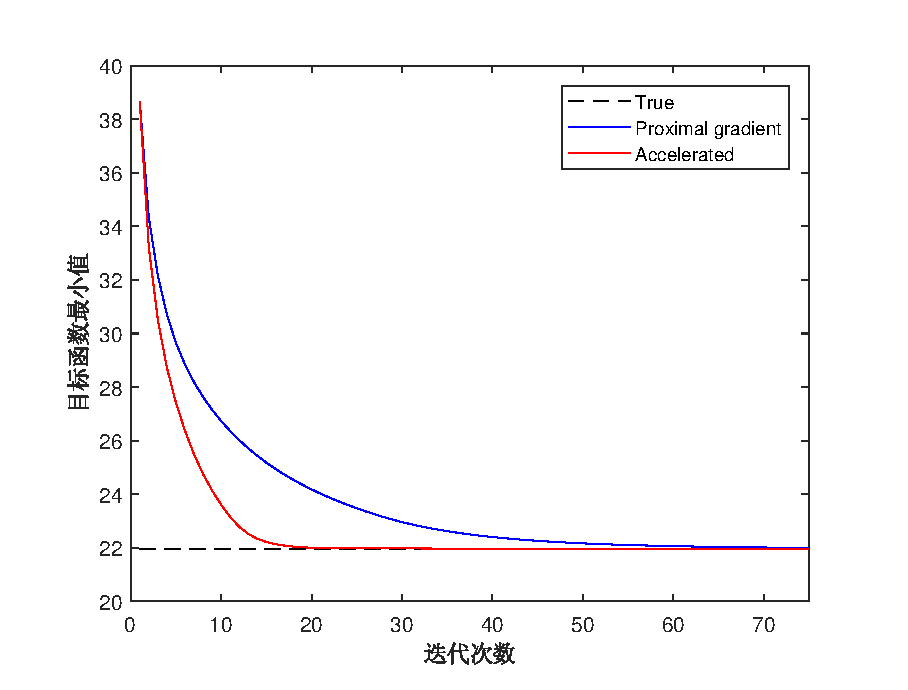
\includegraphics[width=0.6\textwidth]{1.eps}
			\caption{近端梯度算法vs加速近端梯度算法}
		\end{figure}
	\end{frame}
\begin{frame}
	\frametitle{ADMM}
	$$\operatorname{minimize} \quad(1 / 2)\|A x-b\|^{2}+\gamma \|x\|_{1}$$
$$\begin{array}{c}
\operatorname{minimize} \\
\text { subject to } \quad \begin{array}{l}
f(x)+g(z) \\
x-z=0
\end{array} \\
f(x)=(1 / 2)\|A x-b\|^{2} \text { and } g(z)=\gamma\|z\|_{1}
\end{array}$$
	\end{frame}
	\begin{frame}
		\frametitle{ADMM}         % give the algorithm a caption
		$$\begin{aligned}
		x^{k+1} &:=\left(I+\lambda A^{T} A\right)^{-1}\left(z^{k}-u^{k}-\lambda A^{T} b\right) \\
		z^{k+1} &:=\operatorname{prox}_{\lambda \gamma\|\cdot\|_{1}}\left(x^{k+1}+u^{k}\right) \\
		u^{k+1} &:=u^{k}+x^{k+1}-z^{k+1}
		\end{aligned}$$
		\footfullcite{en3}
	\end{frame}
	\begin{frame}[fragile]
	\frametitle{ADMM} 
\begin{algorithm}[H]
	\caption{ADMM}
	\label{alg::conjugateGradient}
	\begin{algorithmic}[1]
		\Require
		$A,x^k,u^k,z^k$\\
		parameter $\lambda,\rho$ \\
		\Repeat \\
	 $x^{k+1} &:=\left(I+\lambda A^{T} A\right)^{-1}\left(z^{k}-u^{k}-\lambda A^{T} b\right)$;
	   \end{algorithmic}
\end{algorithm} 
\footfullcite{en4}
	\end{frame}
		\begin{frame}
		\frametitle{数值实验}
		$\ell_{1}$ -regularized least squares (LS) problem:
		$$\min \left\{\frac{1}{2}\|\mathcal{A} x-b\|^{2}+\gamma\|x\|_{1}\right\}$$
	 我们比较了近端迭代,加速近端迭代,ADMM,CVX来解决这个问题  
	 	\end{frame}
	\begin{frame}
		\frametitle{数值实验}
 参数设置:$$A \in \mathbf{R}^{m \times n},A_{i j} \sim \mathcal{N}(0,1)$$
 $$x^{\text {true }} \in \mathbf{R}^{n},b=A x^{\text {true }}+v,v\in 0.01*(1,m)$$
 $$\gamma=0.1 \gamma_{\max },\gamma_{\max }=\left\|A^{T} b\right\|_{\infty}\footfullcite{en1}$$
近端迭代的参数设置: $\lambda=1$\\
 $\epsilon=10^{-4}$为迭代停止标准\\
	计算平台:IntelCore i5-8265 CPU @1.60GHz  8.00GB RAM Windows10
	\end{frame}
	\begin{frame}
		参数设置:A=500*2500,b=A*x0+v,\\ 其中x0为n*1的稀疏矩阵,密度(在矩阵中非零元素所占的比例):0.05,v为m*1的随机生成的数组
		\begin{figure}[H]
			\centering
			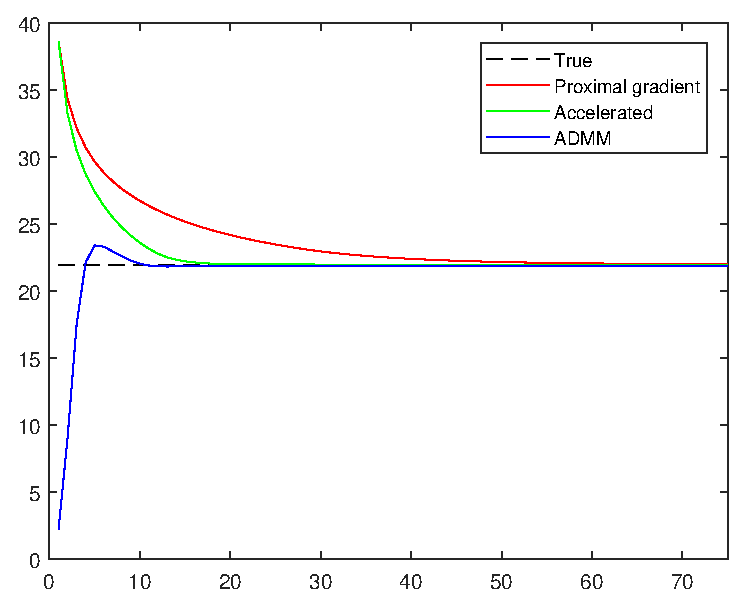
\includegraphics[width=0.6\textwidth]{lasso_comp.eps}
			\caption{Proximal gradient,Accelerated,ADMM}
		\end{figure}
	\end{frame}
	\begin{frame}
		$$\begin{array}{llllll}
		\hline \text { Method } & \text { Iterations } & \text { Time (s) } & p^{\star} & \text { Error (abs) } \\
		\hline \text { CVX } & 15 & 26.53 & 16.5822 & -  \\
		\text { Proximal gradient } & 127 & 0.72 & 16.5835 & 0.09  \\
		\text { Accelerated } & 23 & 0.15 & 16.6006 & 0.26  \\
		\text { ADMM } & 20 & 0.07 & 16.6011 & 0.18 \\
		\hline
		\end{array}$$
			在这个计算中,近端梯度算法迭代较慢,但迭代足够多的次数后,准确性较高,ADMM和加速近端梯度算法虽然迭代次数较少,但得出的值高于真实目标函数的值
	\end{frame}
	
	\begin{frame}
		参数设置:A=1000*3500,b=A*x0+v,\\ 其中x0为n*1的稀疏矩阵,密度(在矩阵中非零元素所占的比例):0.05,v为m*1的随机生成的数组\\
		\begin{figure}[H]
			\centering
			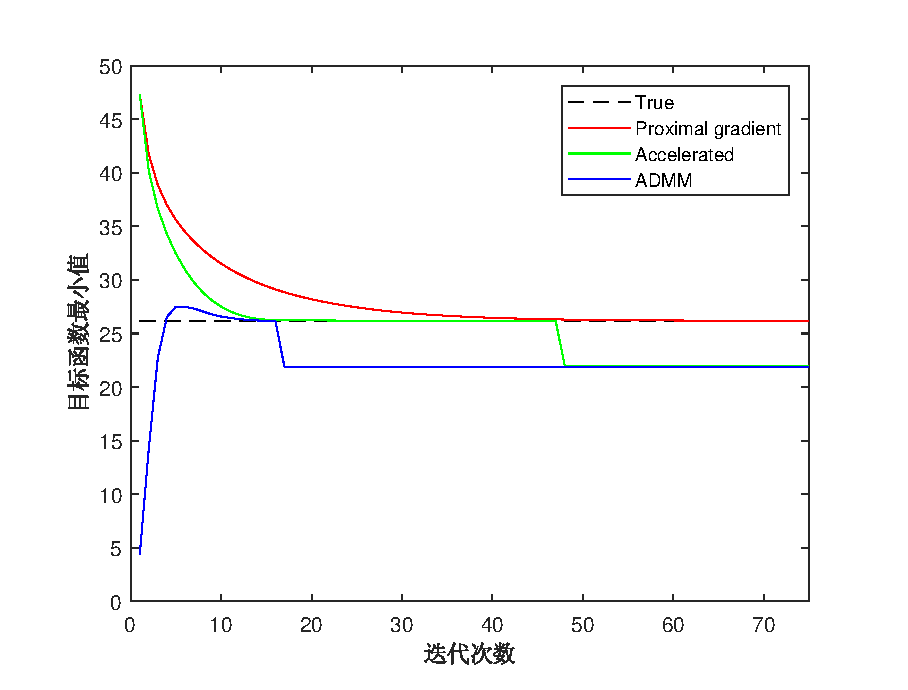
\includegraphics[width=0.6\textwidth]{2.eps}
			\caption{Proximal gradient,Accelerated,ADMM}
		\end{figure}
	\end{frame}
	\begin{frame}
		$$\begin{array}{llllll}
		\hline \text { Method } & \text { Iterations } & \text { Time (s) } & p^{\star} & \text { Error (abs) } \\
		\hline \text { CVX } & 15 & 144.0169 & 23.1788 & -  \\
		\text { Proximal gradient } & 70 & 0.9906 & 23.5835 & 0.05  \\
		\text { Accelerated } & 50 & 0.15 &  26.1053 & 3.16 \\
		\text { ADMM } & 27 & 0.07 & 26.5721 & 3.115  \\
		\hline
		\end{array}$$
			在这个计算中,近端梯度算法迭代较慢,但迭代足够多的次数后,准确性较高,ADMM和加速近端梯度算法虽然迭代次数较少,但得出的低于真实目标函数的值
	\end{frame}
	\begin{frame}
		参数设置:A=600*2000,b=A*x0+v,\\ 其中x0为n*1的稀疏矩阵,密度(在矩阵中非零元素所占的比例):0.05,v为m*1的随机生成的数组
		\begin{figure}[H]
			\centering
			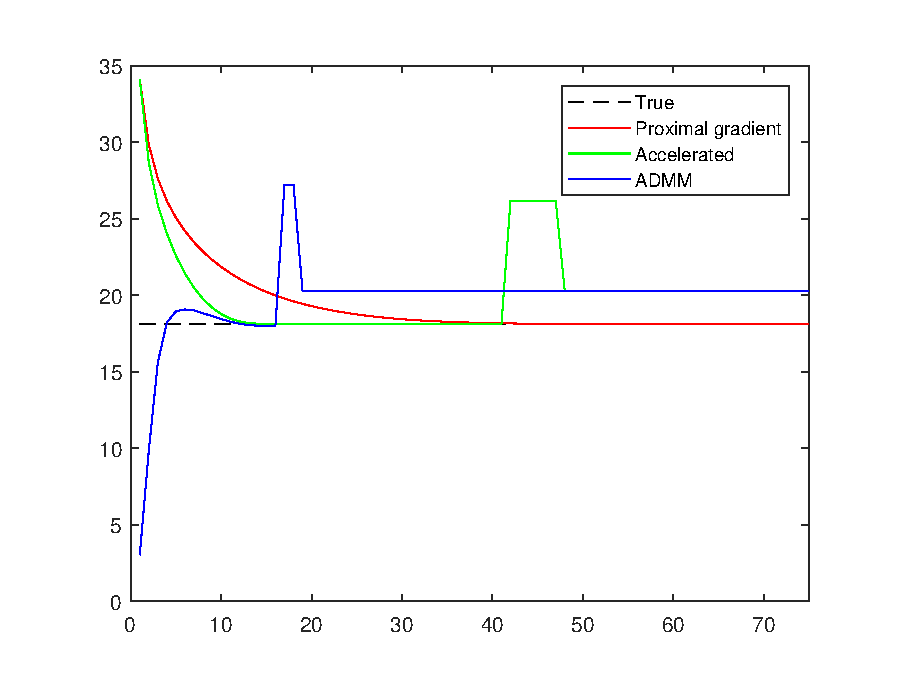
\includegraphics[width=0.6\textwidth]{3.eps}
			\caption{Proximal gradient,Accelerated,ADMM}
		\end{figure}
	\end{frame}
	\begin{frame}
		$$\begin{array}{llllll}
		\hline \text { Method } & \text { Iterations } & \text { Time (s) } & p^{\star} & \text { Error (abs) }  \\
		\hline \text { CVX } & 15 &   27.5314 & 18.5822 & - - \\
		\text { Proximal gradient } & 100 & 0.2774 & 18.5835 & 0.07  \\
		\text { Accelerated } &59 & 0.1559 & 20.6006 & 2.26  \\
		\text { ADMM } & 49 &  0.0589 & 20.6011 & 2.18  \\
		\hline
		\end{array}$$
			在这个计算中,近端梯度算法迭代较慢,但迭代足够多的次数后,准确性较高,ADMM和加速近端梯度算法虽然迭代次数较少,但得出的值高于真实目标函数的值
	\end{frame}
	\begin{frame}
				\frametitle{总结}
\noindent 本文通过三种方式计算lasso问题,并对这三种算法进行介绍,且着重介绍了近端梯度算法及其加速,我们利用数值实验计算来比较三个算法的优缺点。\\
近端梯度算法迭代较慢,但迭代足够多的次数后,准确性较高,ADMM和加速近端梯度算法虽然迭代次数较少,但显示出了较大的误差\\
将三种算法集为一体并进行比较是本文的一大优点,但是由于自身知识面所限,难免会有所错漏,有待改进
	\end{frame}
		\begin{frame}
				\frametitle{小作业分工}
			二分法:\\ 代码编写:李宗翰,袁浩然 ,文档写作:蒋佩禧\\
牛顿迭代法:\\ 代码编写:蒋佩禧,李宗翰,袁浩然 ,文档写作:李宗翰	
					\end{frame}
\begin{frame}[fragile]
\frametitle{迭代法的通用算法}
$$f(x)=x^2-1$$
\begin{lstlisting}
 f=sym('x^2-1');
 [c,E,fc]=newton1(f,0,3,0.005,20);
\end{lstlisting}
$$\begin{array}{lll}
\text { Iter. } & \text { Aprox. } & \text { Error. } \\
\text {  } & 3.0000 & 3.0000 \\
1 & 1.6667 & 1.3333 \\
2 & 1.1333 & 0.5333 \\
3 & 1.0078 & 0.1255 \\
4 & 1.0000 & 0.0078 \\
5 & 1.0000 & 0.0000
\end{array}$$
\end{frame}
\begin{frame}[fragile]
\frametitle{牛顿法vs二分法}
$$12-3 x+2 \cos x=0$$
牛顿法:
$$\begin{array}{|l|l|l|}
\hline \text { 迭代次数 } & \text { 区间值: } \mathrm{b} & \text { 区间值: } \mathrm{a} \\
\hline 1 & 3.43828213866291 & 3.31995568160492 \\
\hline 2 & 3.31995568160492 & 3.34836329704004 \\
\hline 3 & 3.34836329704004 & 3.34741272048233 \\
\hline 4 & 3.34741272048233 & 3.34740283960879 \\
\hline 5 & 3.34741272048233 & 3.34740283960879 \\
\hline
\end{array}$$
\end{frame}
\begin{frame}
\frametitle{二分法}
$$\begin{array}{|l|l|l|}
\hline \text { 迭代次数 } & \text { 区间值: } \mathrm{a} & \text { 区间值: } \mathrm{b} \\
\hline 1 & 3.00000000000000 & 3.50000000000000 \\
\hline 2 & 3.25000000000000 & 3.50000000000000 \\
\hline 3 & 3.25000000000000 & 3.37500000000000 \\
\hline 4 & 3.31250000000000 & 3.37500000000000 \\
\hline 5-13 & \dots & \dots\\
\hline 14 & 3.34735107421875 & 3.34741210937500 \\
\hline 15 & 3.34738159179688 & 3.34741210937500 \\
\hline 16 & 3.34739685058594 & 3.34741210937500 \\
\hline 17 & 3.34739685058594 & 3.34740447998047 \\
\hline 18 & 3.34739685058594 & 3.34740447998047 \\
\hline
\end{array}$$
\end{frame}
\begin{frame}{参考文献}
	\printbibliography
\end{frame}
\end{document}

